\bob{MASALALAR YECHIMI}

\subsection{Masalalar yechimlari}
Quyidagi masalalar yechim yozish tartibini ko’rsatadi. Har bir masalaning
rasmida tanlangan tezlikdagi sarf \eqref{eq:sarf} bog’lanish bilan tasvirlangan;
haqiqiy ishda har biriga o’z shartiga mos alohida chizma tayyorlang.

\noindent\textbf{1-masala.}
Kesim yuzi $S=0.02\,\mathrm{m^2}$ bo’lgan quvurdagi tekis oqimning tezligi
$v=2\,\mathrm{m/s}$. Hajmiy sarfni toping.

\textit{Yechish.} \eqref{eq:sarf} dan foydalanib, berilgan kattaliklarni
bir xil birliklar tizimida qo’yamiz:
\[
  Q = 2\cdot 0.02 = 0.04\,\mathrm{m^3/s}.
\]
\ref{fig:masala1}-rasmdagi belgilangan nuqta shu natijani ko’rsatadi.

\noindent\textbf{Javob:} $Q=0.04\,\mathrm{m^3/s}$.

\begin{figure}[htbp]
  \centering
  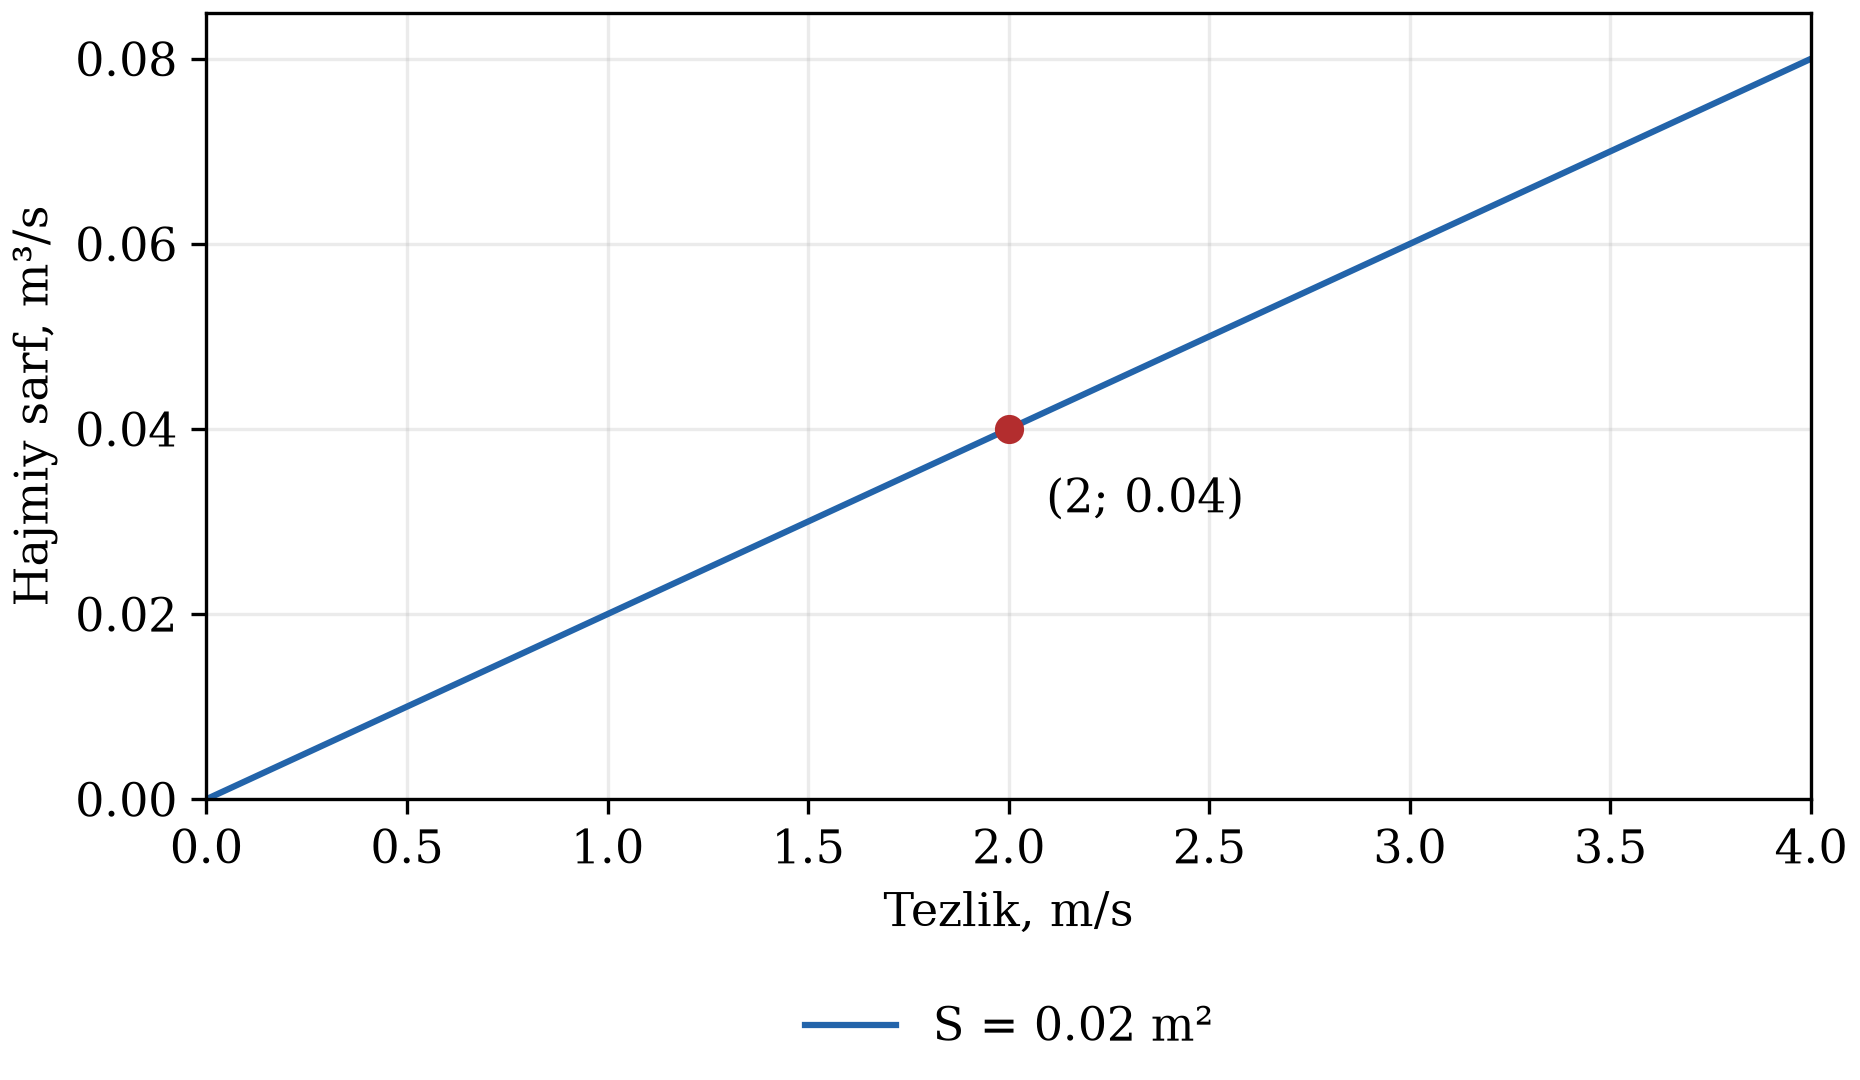
\includegraphics[width=0.65\textwidth]{namuna.png}
  \caption{1-masala: tezlik va hajmiy sarf orasidagi bog’lanish}
  \label{fig:masala1}
\end{figure}

\noindent\textbf{2-masala.}
Birinchi masaladagi oqimning zichligi $\rho=1000\,\mathrm{kg/m^3}$.
Massa sarfini aniqlang.

\textit{Yechish.} Birinchi masalada $Q=0.04\,\mathrm{m^3/s}$ topildi.
\eqref{eq:massa} ga ko’ra,
\[
  \dot{m} = 1000\cdot 0.04 = 40\,\mathrm{kg/s}.
\]
Natijani \eqref{eq:umumiy} orqali ham tekshirish mumkin:
$1000\cdot 2\cdot 0.02=40$.
\ref{fig:masala2}-rasmdagi sarf zichlikka ko’paytiriladi.

\noindent\textbf{Javob:} $\dot{m}=40\,\mathrm{kg/s}$.

\begin{figure}[htbp]
  \centering
  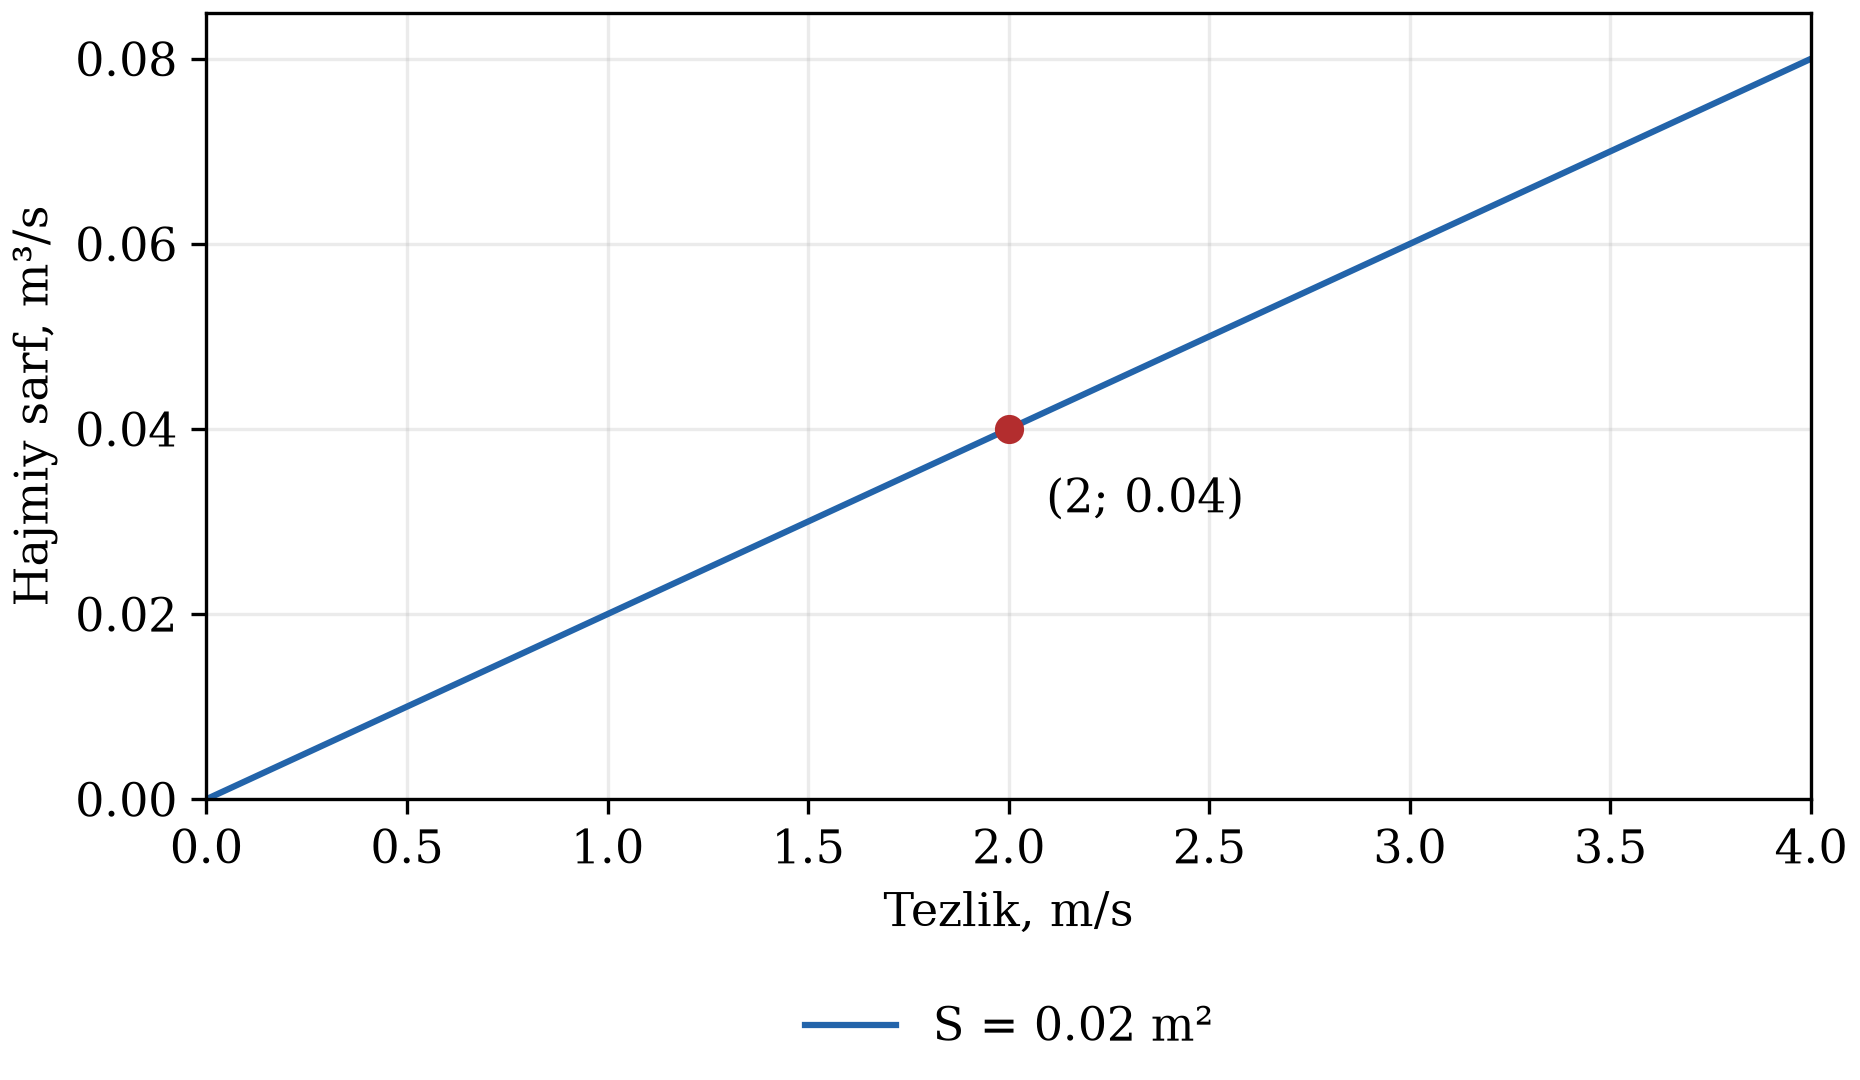
\includegraphics[width=0.65\textwidth]{namuna.png}
  \caption{2-masala: massa sarfini hisoblash uchun hajmiy sarf}
  \label{fig:masala2}
\end{figure}

\subsection{Natijalar jamlanmasi}
\ref{tab:javoblar}-jadvaldagi natijalar shablon misollariga tegishli.
Qo’llanma bilan solishtirish ustunini haqiqiy javob tekshirilgach to’ldiring;
farq bo’lsa uning sababini masala yechimida \textit{Izoh.} bilan tushuntiring.

\begin{table}[htbp]
  \centering
  \caption{Namunaviy masalalarning javoblari}
  \label{tab:javoblar}
  \begin{tabular}{|c|l|p{5.5cm}|}
    \hline
    № & Javob & Qo’llanma bilan \\
    \hline
    1 & $Q=0.04\,\mathrm{m^3/s}$ & [Solishtirishni kiriting] \\
    2 & $\dot{m}=40\,\mathrm{kg/s}$ & [Solishtirishni kiriting] \\
    \hline
  \end{tabular}
\end{table}
